\section{Wnioski}
\indent W celu analizy porównawczej sygnałów uzyskanych na wyjściu z przetwornika DAC oraz sygnałów wzorcowych wygenerowanych w środowisku Matlab zapisano przesłane na oscyloskopie przebiegi czasowe w formacie danych *.CSV. Następnie importując je do środowiska Matlab możliwe było przeskalowanie wcześniej wygenerowanych przebiegów wzorcowych. Po przeskalowaniu i dopasowaniu fazy możliwe było zestawienie na jednym wykresie syganłów zadanych oraz sygnałów wygenerowanych przez układ. Wyniki kilku eksperymentów przedstawione są na rysunkach \ref{fig:10_100}, \ref{fig:10_100_1000} i \ref{fig:50_60}, gdzie kolorem niebieskim zaznaczony jest przebieg wygenerowany przez układ, natomiast kolorem czerwonym przebieg wzorcowy. Parametry podane jako wejście do układu zestawione zostały w tabelach \ref{tab_10_100}, \ref{tab_10_100_1000} i \ref{tab_50_60}.

\begin{table}[h]
	\caption{Parametry pierwszego przebiegu.}
	\label{tab_10_100}
	\centering
	
	\begin{tabular}{|c|c|c|}
		\hline
		\textbf{Częstotliwość [Hz]} & \textbf{Amplituda} & \textbf{Przesunięcie fazowe [\textdegree]}\\
		\hline
		10 & 7 & 180 \\
		\hline
		100 & 2 & 0 \\
		\hline
	\end{tabular}
\end{table}

\begin{figure}[h!]
	\centering
	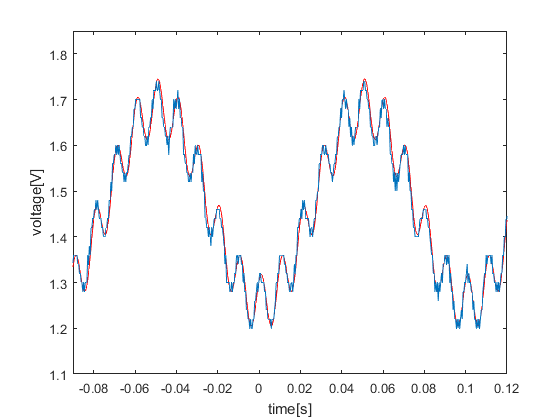
\includegraphics[scale = 0.8]{fig/10_100.png}
	\caption		
	{Zestawienie przebiegu wygenerowanego przez układ z przebiegiem wzorcowym dla parametrów z tabeli \ref{tab_10_100}.}
	\label{fig:10_100}
\end{figure}

\begin{table}[h]
	\caption{Parametry drugiego przebiegu.}
	\label{tab_10_100_1000}
	\centering
	
	\begin{tabular}{|c|c|c|}
		\hline
		\textbf{Częstotliwość [Hz]} & \textbf{Amplituda} & \textbf{Przesunięcie fazowe [\textdegree]}\\
		\hline
		10 & 7 & 180 \\
		\hline
		100 & 2 & 0 \\
		\hline
		1000 & 2 & 0 \\
		\hline
	\end{tabular}
\end{table}

\begin{figure}[h!]
	\centering
	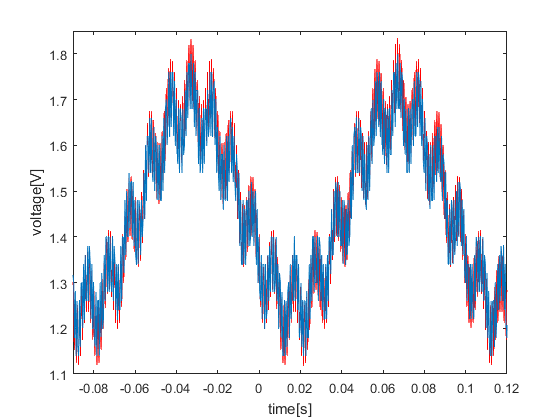
\includegraphics[scale = 0.8]{fig/10_100_1000.png}
	\caption		
	{Zestawienie przebiegu wygenerowanego przez układ z przebiegiem wzorcowym dla parametrów z tabeli \ref{tab_10_100_1000}}
	\label{fig:10_100_1000}
\end{figure}

\begin{table}[h]
	\caption{Parametry trzeciego przebiegu.}
	\label{tab_50_60}
	\centering
	
	\begin{tabular}{|c|c|c|}
		\hline
		\textbf{Częstotliwość [Hz]} & \textbf{Amplituda} & \textbf{Przesunięcie fazowe [\textdegree]}\\
		\hline
		50 & 4 & 180 \\
		\hline
		60 & 3 & 90 \\
		\hline
	\end{tabular}
\end{table}

\begin{figure}[H]
	\centering
	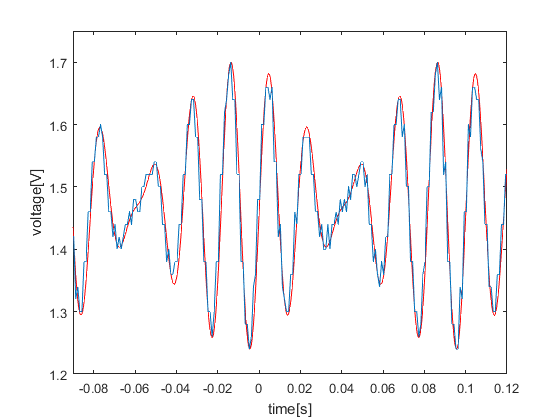
\includegraphics[scale = 0.8]{fig/50_60.png}
	\caption		
	{Zestawienie przebiegu wygenerowanego przez układ z przebiegiem wzorcowym dla parametrów z tabeli \ref{tab_50_60}}
	\label{fig:50_60}
\end{figure}

\indent Analizując przedstaione wyniki można zauważyć stosunkowo dobre dopasowanie wygenerowanych sygnałów do sygnałów wzorcowych. Widoczne na wykresie \ref{fig:50_60} ostre zmiany wartości wyjściowej tłumaczyć można jako niedokładność generowaną na zbliżeniu przez oscyloskop. Rozdzielczość, w której zapisane zostały serie danych wynosi 600x600 co generuje widoczne niedokładności.

\indent W ogólnym rozrachunku udało się zrealizowac wszystkie założenia projektowe. Realizację algorytmu genaracji sygnału na podstawie danych parametrów. Wysyłanie wyliczonych wartości na układ DAC. Interfejs użytkownika umożliwiający zadawanie parametrów sygnału oraz komunikację z mikrokontrolerem.